\documentclass[12pt,halfline,a4paper]{ouparticle}
\usepackage[english]{babel}
\usepackage[colorlinks=true,citecolor=blue,linkcolor=blue,urlcolor=blue,hyperfootnotes=false]{hyperref}
\usepackage{natbib}
\usepackage[utf8]{inputenc}
\usepackage{booktabs}
\usepackage{multirow}
\usepackage[dvipsnames]{xcolor}
\usepackage{marvosym}
\usepackage{fontawesome}
\usepackage[bottom]{footmisc}

\usepackage{silence}
%% \WarningFilter{latex}{Text page 6 contains only floats}

\usepackage[T1]{fontenc}
%% \usepackage{tipa}

\begin{document}

\title{Ministerial Stability During Presidential Approval Crises: The Moderating Effect of Ministers’ Attributes on Dismissals in Brazil and Chile\thanks{This research has been funded by the Chilean National Agency for Research and Development (ANID/PFCHA/72200340). Acknowledgements to a number of scholars and colleagues can be found at the end of the document. The author declares no potential conflict of interest with respect to this research.}}

\author{%
\name{Bastián González-Bustamante\thanks{{\faMapMarker} St Hilda's College, Cowley Place, Oxford {\scriptsize OX4 1DY}, {\large \Letter} \href{mailto:bastian.gonzalezbustamante@politics.ox.ac.uk}{bastian.gonzalezbustamante@politics.ox.ac.uk}, {\large \Letter} \href{mailto:bastian.gonzalez.b@usach.cl}{bastian.gonzalez.b@usach.cl}, {\faHome} \href{https://bgonzalezbustamante.com/}{https://bgonzalezbustamante.com}, {\scriptsize ORCID iD} \href{https://orcid.org/0000-0003-1510-6820}{https://orcid.org/0000-0003-1510-6820}.}}
\address{University of Oxford \\ Universidad de Santiago de Chile}
%% \email{bastian.gonzalezbustamante@politics.ox.ac.uk}
%% \and
%% \name{Co-Author}
%% \address{Affiliation}
%% \email{Email}
}

\abstract{This paper analyses the effect of ministers’ exposure to periods of low presidential approval in Brazil and Chile between 1990 and 2014. Approval is explored with quarterly estimates using a dyad-ratios algorithm and merged into a time-dependent cabinet data set to evaluate individual ministerial terminations ($N$ = 4,245). The empirical strategy combines time-varying exposure Cox regressions with observational data and propensity score and matching to estimate the effect of low approval on ministerial survival and perform a moderation analysis with three profiles associated with presidential strategies: (i) nonpartisan ministers to limit agency loss and moral hazard; (ii) economists as ministers to optimise cabinet performance and send positive signals to the electorate; and (iii) party leaders as ministers to optimise legislative support. The main findings show that risk increases by 135.1\% in periods of low approval. In addition, approximately only one in five nonpartisan ministers is removed compared to party members.}

%% \date{\today}
\date{{\normalsize October 2, 2022} \\ {\footnotesize This article has been accepted in the {\itshape British Journal of Politics and International Relations}}}

\keywords{ Brazil; cabinets; Chile; ministerial turnover; presidential approval; propensity score; survival analysis}

\maketitle

\section{Introduction}
\label{sec1}

In May 2010, just a month after the start of Sebasti\'an Pi\~nera’s first presidential term, Jaime Ma\~nalich, the recently appointed health minister, was summoned to testify about an allegedly falsified alcohol test performed seven months earlier on Pi\~nera’s brother after a traffic accident. The test took place at a private clinic where Ma\~nalich was then general manager and Pi\~nera was a shareholder. Regardless of public pressure, Ma\~nalich remained health minister throughout the four-year administration. A very different situation occurred in June 2020, when Pi\~nera made the fourth cabinet change of his second term (2018-2022). Despite persistent questioning of the government’s response to the coronavirus pandemic, the change consisted only in a reshuffle of the same ministers, designed partly to protect questioned Health Minister Jaime Ma\~nalich. The protagonists are the same as in 2010 but the outcome was entirely different: only nine days after the reshuffle, Ma\~nalich resigned in the face of criticism of the inefficiency of the dynamic quarantines implemented by the government and a mismatch between the statistics reported by the Health Ministry and the World Health Organization (WHO). Thus, while the President was again willing to protect Ma\~nalich, the pressure was unsustainable.

This case is an excellent example of how a president can protect ministers from calls for their resignation and the effect of scandals. In this particular example, Pi\~nera reappointed Ma\~nalich as a minister in his second term but, this time, was unable to protect him. Moreover, this is a case of a nonpartisan minister close to the president and illustrates how a president can limit moral hazard and agency loss by appointing and protecting independent ministers close to his entourage or inner circle and without partisan loyalties.

While ministers’ attributes and trajectories are a recurrent topic of study from different approaches, theoretical arguments tend to result in a conceptual heterogeneity that complicates empirical research \citep{Camerlo2018}. This heterogeneity translates into a variety of concepts for identifying profiles that are complex to measure empirically, posing a methodological challenge for testing how ministers’ profiles offer advantages in the face of unexpected events or shocks that impact governments’ stability. In this context, we consider periods of low presidential approval, a situation common to almost every administration that should impact actors’ incentives and strategies. 

Thus, our main question is: How can a minister’s attributes prevent his exit from the cabinet during periods of low presidential approval? Answering this question allows us to offer an empirically approachable conceptualisation of ministerial profiles linked to presidential strategies in contexts of approval crises and, in this way, make a theoretical contribution to bridging the gap in the general conceptualisation of profiles. In addition, we propose a specific procedure for correctly estimating effects and bias using the survival approach, which constitutes a substantial, novel methodological contribution. This contribution is relevant since straightforward modelling of the relationship between low approval and cabinet turnover may be biased and exposed to endogeneity because presidents or prime ministers tend to reshuffle their cabinets at times of low popularity \citep{Kam2005, MartinezGallardo2014}.

We will refer to two country-specific cases: Brazil and Chile. Although both are cases of multi-party coalitions, political alliances in Chile have been remarkably stable in recent decades and, for instance, Chile has more robust party organisation capabilities \citep{Martinez2021}. In addition, both cases have shown a higher degree of technical control over economic policies in recent decades compared to other countries in the region, such as Argentina, where technocracy has gradually declined \citep{Dargent2015}. Finally, as evidenced below, both countries have experienced periods of low presidential approval and comparable levels of ministerial survival in the medium to long term.

In the next section, we present the theory and empirical expectations, reflecting first on stochastic events, low approval and ministerial recruitment before going on to connect recruitment and political careers with different ministers’ profiles and principal-agent, signalling and coalition theories. We then present our empirical strategy with the encoding of the time-dependent data set, detailed information on the regressions with observational data and the application of propensity score and matching along with placebo tests and robustness checks. The main results are then presented with the estimation of the effect of exposure to low approval on the exit of cabinet ministers, moderation analyses and additional tests. Finally, the main findings are summarised and briefly discussed.

\section{Ministerial Turnover and Ministers’ Profiles}
\label{sec2}

\subsection{Stochastic Events, Low Approval and Ministerial Recruitment and Careers}
\label{sec2.1}

The concept of crisis is associated with stochastic events in the framework of the event-based approach in government survival literature, especially in the case of parliamentary systems \citep{Browne1986, Fortunato2018, King1990, Warwick1994}. This concept accounts for unforeseen events or shocks that affect the stability of governments. The magnitude of their effect depends on different factors, such as the complexity of the bargaining environment and the party system’s characteristics. More complex environments render governments more sensitive to these events \citep{Chiba2015, Laver1996, Laver1990}. Such events can be critical and generate a renegotiation of the balance of power as it stood at the beginning of a presidential term and may even lead to a reordering of parties and coalitions. Both situations can, in turn, trigger a cabinet reshuffle \citep{MartinezGallardo2012}.

Events that typically affect cabinet stability include protests, economic crises, media scandals, corruption cases, low approval and natural disasters of different sorts \citep{Camerlo2015a, MartinezGallardo2014}. It is to be expected that different events will have different effects on the actors’ behaviour depending on the specific context. However, as \cite{Berlinski2010} indicate, evaluating all possible random shocks is empirically complex and we, therefore, opted to focus on periods of low presidential approval.

In these periods, a president should have incentives to correct drops in her\footnote{The use of pronouns follows the standard in principal-agent literature: feminine for the principal and masculine for the agent.} approval by making cabinet changes and firing inefficient ministers or those whose profile does not tally with strategic presidential decisions, in a similar fashion to what happens with prime ministers in parliamentary systems \citep{Dewan2005, McAllister2003}. 

Presidential approval dynamics tend to follow a cyclical model with quadratic patterns: a honeymoon period just after the election, a gradual deterioration, and a slight recovery towards the end of the term \citep[][see also \citeauthor{Brace1992}, \citeyear{Brace1992}; \citeauthor{Carlin2018}, \citeyear{Carlin2018}]{Stimson1976}. In Latin American countries, the evidence confirms a significant honeymoon effect during the first three quarters of an administration, followed by a deterioration to a low of 40-45\% approval and, finally, a slight recovery \citep{Carlin2019b, Carlin2018}.

Consequently, our first empirical expectation is that presidents do indeed carry out reshuffles in a bid to counter periods of low approval. Therefore, we formulate the following hypothesis:

\begin{itemize}
\item{{\itshape Low Approval Hypothesis.} Exposure to periods of low presidential approval increases the likelihood that a minister will be removed from the cabinet.}
\end{itemize}

Our argument and empirical expectation are straightforward: low approval increases the likelihood of the dismissal of ministers. This viewpoint differs slightly from \cite{Camerlo2015b} since, albeit asserting that portfolio reallocation is mediated by approval, they also suggested that partisan ministers choose to leave the cabinet when the government is unpopular and presidents command only the loyalty of their inner circle. In other words, presidents do not fire ministers in turbulent times but are abandoned by them. We suspect this idea is driven by the Argentine single-party government case, which these authors analysed. In multi-party coalitions, a failure to renegotiate the initial equilibrium of the coalition could imply the parties’ abandonment of the government \citep{MartinezGallardo2012}. In this case, their abandonment of the president should trigger a major change in the bargaining environment and a new government coalition, not just a cabinet reshuffle.

At this point, we nuance our argument by incorporating the idea that specific ministers’ profiles and attributes can temper or moderate the presidential decision to dismiss them because specific profiles are linked to identifiable presidential strategies. Therefore, we are particularly interested in testing the protective effect of some traits linked to specific strategies. To support this argument, we examine some theoretical perspectives related to ministerial recruitment and the political career concept. 

Ministerial recruitment in European parliamentary systems has been studied extensively by, for example, \cite{Blondel1988}, \cite{Blondel1997} and \cite{Blondel1991}. According to \cite{Camerlo2018}, this work is related to studies of trajectories and circulation of the elite. From the standpoint of the study of political elites, recruitment can be understood as a process of selecting citizens with sufficient motivation and social advantages to attain important positions \citep{Putnam1976}. In this vein, recruitment is intrinsically linked to a ministerial career as part of an individual’s political career. A ministerial career can be defined as the time between a minister’s first appointment to the cabinet and his final departure from the government \citep{RodriguezTeruel2011}. In this sense, ministers’ careers may be dynamic, and their departure from the cabinet may not be synonymous with the end of their political career. In their analysis of European parliamentary cabinets, \cite{Blondel1993, Blondel1997} conclude that ministers’ careers do not terminate when they leave office and they generally move to other important public positions or positions that, albeit less prominent publicly, are important in professional terms. In some cases, they also subsequently return to the cabinet \citep{GonzalezBustamante2018}. In Latin America, ministers with higher levels of political capital are, in general, less likely to face abrupt removal from office \citep{EscobarLemmon2005, EscobarLemmon2009}.

Political careers can be explained using structuralist, interactionist or motivational approaches \citep{Alcantara1997}. The structuralist approach focuses on the effect of individuals’ background, social capital and academic credentials on their access to positions of power, while the interactionist approach emphasises processes of interaction associated with the political circumstances in which individuals operate. Finally, the motivational approach attempts to explain their interests and strategies at different stages of their political career as conditioned by individual ambition in accordance with the classic concept of \cite{Schlesinger1966}.

The structuralist approach can be related to a series of studies that have focused precisely on individuals’ educational background and academic credentials. Examples include the work of \cite{EscobarLemmon2016} and \cite{AiCamp1995, AiCamp2002} on the advantages that academic credentials and family ties confer in obtaining positions of privilege in the Mexican elite. These studies tend to connect with specific sociological approaches suggesting that individuals’ political trajectories are conditioned by their resources and capital \citep{Joignant2012} and that political capital operates symbolically based on recognition \citep{French2011}.

At this point, it is possible to note that both ministerial recruitment and the political career concept have been strongly influenced by approaches based on the characteristics of individuals, resembling sociological perspectives. This influence is associated with an important drawback. These approaches do not constitute a homogeneous theoretical body and, as pointed out by \cite{Camerlo2018}, this makes it difficult to work empirically with their conceptualisations. Indeed, some of these approaches use professional politician, outsider, specialist or generalist concepts and nuanced measurements based on fuzzy-set theory \citep{Camerlo2015b}. Moreover, when the sociological approach based on resources and capital is incorporated \citep{Joignant2011, Joignant2012}, an overwhelming number of subtypes of politicians, technocrats and technopols can be identified and, strictly speaking, these can be too fuzzy for empirical analysis. 

In light of these difficulties, we look at potential connections between individual attributes and ministerial profiles using approaches such as principal-agent perspectives, signalling and coalition studies that allow us to explore specific presidential strategies in crisis contexts.

\subsection{Nonpartisan Ministers, Technocrats and Party Leaders}
\label{sec2.2}

A number of studies have suggested that presidential cabinets are lighter on party members than parliamentary cabinets and that there is not necessarily a correlation between parties’ representation in the cabinet and the seats they hold in Congress. This reflects presidents’ high autonomy in choosing their ministers, which they exercise to appoint nonpartisan ministers \citep{Altman2000, Altman2008}. Indeed, the appointment of nonpartisan ministers can be understood as a presidential strategy to control moral hazard problems and the risk of agency loss \citep{Chaisty2018, MartinezGallardo2015}. This situation can be remarkably delicate in multi-party systems, although the institutional architecture of presidentialisms should allow the principal -- in this case, the president -- to exercise better control of moral hazard in the chain of delegation with her ministers. Thus, we propose the following hypothesis:

\begin{itemize}
\item{{\itshape Nonpartisan Hypothesis.} Nonpartisan ministers are less likely to be removed from the cabinet during periods of low presidential approval.}
\end{itemize}

Conversely, classifying all a president’s non-legislative support simply as nonpartisan can be too general and imprecise, creating a gap between studies of cabinet formation and ministerial recruitment. \cite{MartinezGallardo2015} and \cite{Camerlo2018} suggest that, to bridge this gap, the recruitment of nonpartisan ministers should be considered a strategic decision on the part of a president in order to address crises and particular circumstances.

In a similar vein, and in combination with signalling theorising, incentives operate in the second chain of delegation in presidential democracies, where the president is an agent of the electorate \citep{Elgie2020}. In this chain, the president has incentives to limit moral hazard and ensure ministers perform adequately in order to send signals to the electorate and increase presidential popularity. These incentives should be more substantial when re-election is permitted \citep[][see also \citeauthor{Beckman2020}, \citeyear{Beckman2020}]{Camerlo2015a}. They also enable us to reinterpret the role of expertise in the cabinet. Our argument does not explain the supremacy of technocracy and the role of economists only in terms of socio-historical processes but rather the opportunity they offer the president to show good results and send adequate signals to the electorate for the sake of the party’s or coalition’s continuity in government or with the aim of obtaining re-election. 

In Latin America, ministers’ profiles have been studied in the context of the appointment in the 1990s of technocrats, who can also be classified as nonpartisan ministers \citep[][see also \citeauthor{Camerlo2018}, \citeyear{Camerlo2018}; \citeauthor{Joignant2011}, \citeyear{Joignant2011}]{Centeno1998, Silva2009}. Their emergence reflected the specific socio-historical circumstances of the region’s democratisation, the influence of the World Bank’s first-generation reforms and the recommendations of the Washington Consensus, which tended to foster significant changes in the ministerial recruitment process, consolidating the role of technocrats in public policymaking \citep{Camerlo2018, Centeno1998}. Technocrats have since gone on to play a leading role in political and economic transformations in Latin America \citep{Centeno1998, Silva2009}. 

The World Bank reforms boosted the New Public Management (NPM) approach in the region, fostering a clear-cut separation between politics and administration. This separation was accompanied by a critical view of the balance between patronage and merit-based appointments in the executive \citep{GonzalezBustamante2020}. This view was also driven partly by the World Bank’s second-generation reforms, which focused on professionalising civil services and reforming the public administration to make it more meritocratic \citep{Panizza2005}.

Therefore, it is possible to observe a change in patronage systems depending on the hierarchical level and the cohabitation of politicians with technocrats at the highest levels of the executive \citep{Panizza2019}. Indeed, not all patronage appointments are clientelist in nature and some have other purposes \citep{Kopecky2016}. For example, \cite{Panizza2018} propose a taxonomy of patronage practices that identifies different types of motivations for appointments used to reward and maintain a network of political activists:  to provide technical expertise, to control the public bureaucracy, to secure support for policy initiatives and to gather electoral support. The appointment of technocrats or technopols at the higher level of the executive is associated precisely with the need for technical expertise \citep[see also][]{Joignant2011, Dargent2015}.

We evaluated technical knowledge as a desirable trait in a presidential cabinet since it can help to manage difficult moments and promote the government agenda. Indeed, the high levels of expertise required by some ministries can make it more difficult to replace the incumbent minister \citep{MartinezGallardo2014}. We are specifically interested in the role played by economists, given the abundant literature on the influence of the technocratic phenomenon in Latin America \citep[][see also \citeauthor{Camerlo2018}, \citeyear{Camerlo2018}]{Centeno1998, Silva2009}. However, given that not all countries have experienced a clear hegemony of technocracy and, particularly, of economists \citep{Dargent2015}, we also use robustness checks to test alternative measures of expertise such as the technopol profile \citep{GonzalezBustamante2018, Joignant2011} and the holding of a PhD \citep{Camerlo2015b}. The argument is that a more technical cabinet allows presidents to obtain good results in implementing public policies and send signals to the electorate through which to maintain or regain their popularity. Therefore, our empirical expectation is as follows:

\begin{itemize}
\item{{\itshape Technocracy Hypothesis.} Ministers who are economists are less likely to be removed from the cabinet during periods of low presidential approval.}
\end{itemize}

Finally, the role of party leaders or political capital can be understood as a mediating factor in power balances in a multi-party system or even in single-party governments in the framework of relations between the executive and the legislature. Rather than the symbolic dimension of political capital, we highlight the argument that cabinet allocation can be used strategically to negotiate with parties \citep{Schleiter2020}. In this sense, appointing and protecting ministers who are party leaders can be analogous or complementary to the strategy of forming coalitions to circumvent legislative blockages \citep{AmorimNeto2006, MartinezGallardo2012}. This strategy operates in the opposite way to the limiting of agency loss through the appointment of nonpartisan ministers close to the president: it may increase moral hazard but may also translate into explicit legislative support \citep{Altman2000, AmorimNeto2006}.

A side effect of the increased moral hazard may be the extension of the patronage system to the highest levels of the civil service. For example, the politicisation of senior civil servants tends to be higher in ministries than in government agencies \citep{Bach2020}. Moreover, \cite{Staronova2021} show that senior civil servants are more likely to be replaced after a cabinet reshuffle, which is consistent with politicisation of the civil service. Similarly, \cite{GonzalezBustamante2020} shows high turnover rates among senior civil servants, comparable to those seen in the cabinet.

Despite these negative externalities, a president may need political support and, in this context, being a party leader could also offer ministers protection since it implies an ability to mobilise support and affect the negotiation environment and, consequently, the president’s legislative strategy. Indeed, ministerial appointments of party leaders could be used as a strategy to negotiate legislative support \citep{Schleiter2020}. Consequently, we pose the following hypothesis:

\begin{itemize}
\item{{\itshape Political Capital Hypothesis.} Ministers who are party leaders are less likely to be removed from the cabinet during periods of low presidential approval.}
\end{itemize}

\section{Empirical Strategy}
\label{sec3}

\subsection{Time-Dependent Data Encoding}
\label{sec3.1}

Our empirical strategy combines time-varying exposure survival models, propensity score analysis and matching techniques. Several recent studies of ministerial duration and turnover have adopted this approach \citep{Berlinski2007, Berlinski2010, Camerlo2015a, Kerby2015, MartinezGallardo2014, QuirozFlores2015}. However, these models are not exempt from the problem of non-random selection inherent to observational data. We, therefore, combine propensity score and matching estimation in order to estimate correctly the effect of presidential approval crises on the departure of cabinet ministers and the possible moderating effect of certain specific profiles and attributes.

First, we merged the data sets of \cite{Franz2016} and \cite{GonzalezBustamante2022} about ministers in Brazil and Chile between 1990 and 2014. Both sets contain information about the ministers’ attributes and trajectories and the exact dates on which they became and ceased to be ministers, which are particularly important for our empirical strategy. We thereby obtained a set of 488 observations that we coded as a time-dependent data set with quarterly cut-off points for the whole period in order to incorporate presidential approval and macroeconomic data as time-varying covariates.

For this procedure, we used the time-interval model of \cite{Therneau2020} in which the base is encoded with cases that have multiple observations -- in this case, $i$-$th$ ministers -- according to defined time intervals corresponding to the four quarters of each year ($q_{1}$, $q_{2}$, $q_{3}$, $q_{4}$). Therefore, we generated a time event $T$ considering each interval $q_{j}$ and taking into account the individual ministerial terminations $Y_{i}$ by constructing intervals where $Z(t) = I(t > Y_{i})$.

The variance of the time-varying covariates is coded over the closed interval, that is, at the end of each quarter. It is then possible to observe the different covariates $X_{j[i]}$ in each quarter, and the last interval of each case ends with the departure of the minister $Y_{i}$. Accordingly, we merge in each interval $Z(t)$ quarterly smoothed presidential approval with \cite{Carlin2019} data.\footnote{This data set contains 46,008 survey marginal time series in 47 countries calculated with \citeauthor{Stimson2018}’s (\citeyear{Stimson2018}) dyad-ratios algorithm. We use quarterly smoothed presidential approval from Brazil and Chile as a more consistent data point than the average value \citep{Stimson2018}. It is important to note that quarterly unsmoothed and smoothed approval are correlated at 0.99 \citep{Carlin2018}.}

In addition, we merged \citeauthor{WorldBank2020} macroeconomic indicators (\citeyear{WorldBank2020}; see also \citeauthor{Piburn2020}, \citeyear{Piburn2020}) and the legislative effective number of parties (ENP) with the \cite{Gallagher2005} indicator updated for the period between 1990 and 2014, derived from the original measurements of \cite{Laakso1979} and \cite{Gallagher1991}. The macroeconomic indicators that are merged into the set are GDP growth, measured as the annual percentage per capita change, and inflation, measured as the annual change in consumer prices. The code programmed to encode the data set and replicate the main article analyses is available in the \href{https://osf.io/asgbj/?view_only=144acd6c8eca4836880b57dee85ea4ff}{Supplementary Material}.

This procedure allowed us to obtain a set of 4,245 observations to which we applied administrative censoring in the final interval when it coincided with the end of the corresponding presidential term. \textcolor{blue}{Figure} \ref{FIG1} shows a nonparametric Kaplan-Meier estimation based on individual ministerial terminations and a LOESS estimation of presidential approval between 1990 and 2014 in both countries.

\begin{figure}[h]
\caption{Kaplan-Meier Survival Estimations for Ministers and Presidential Approval in Brazil and Chile}
\label{FIG1}
\centering \vspace{2mm}
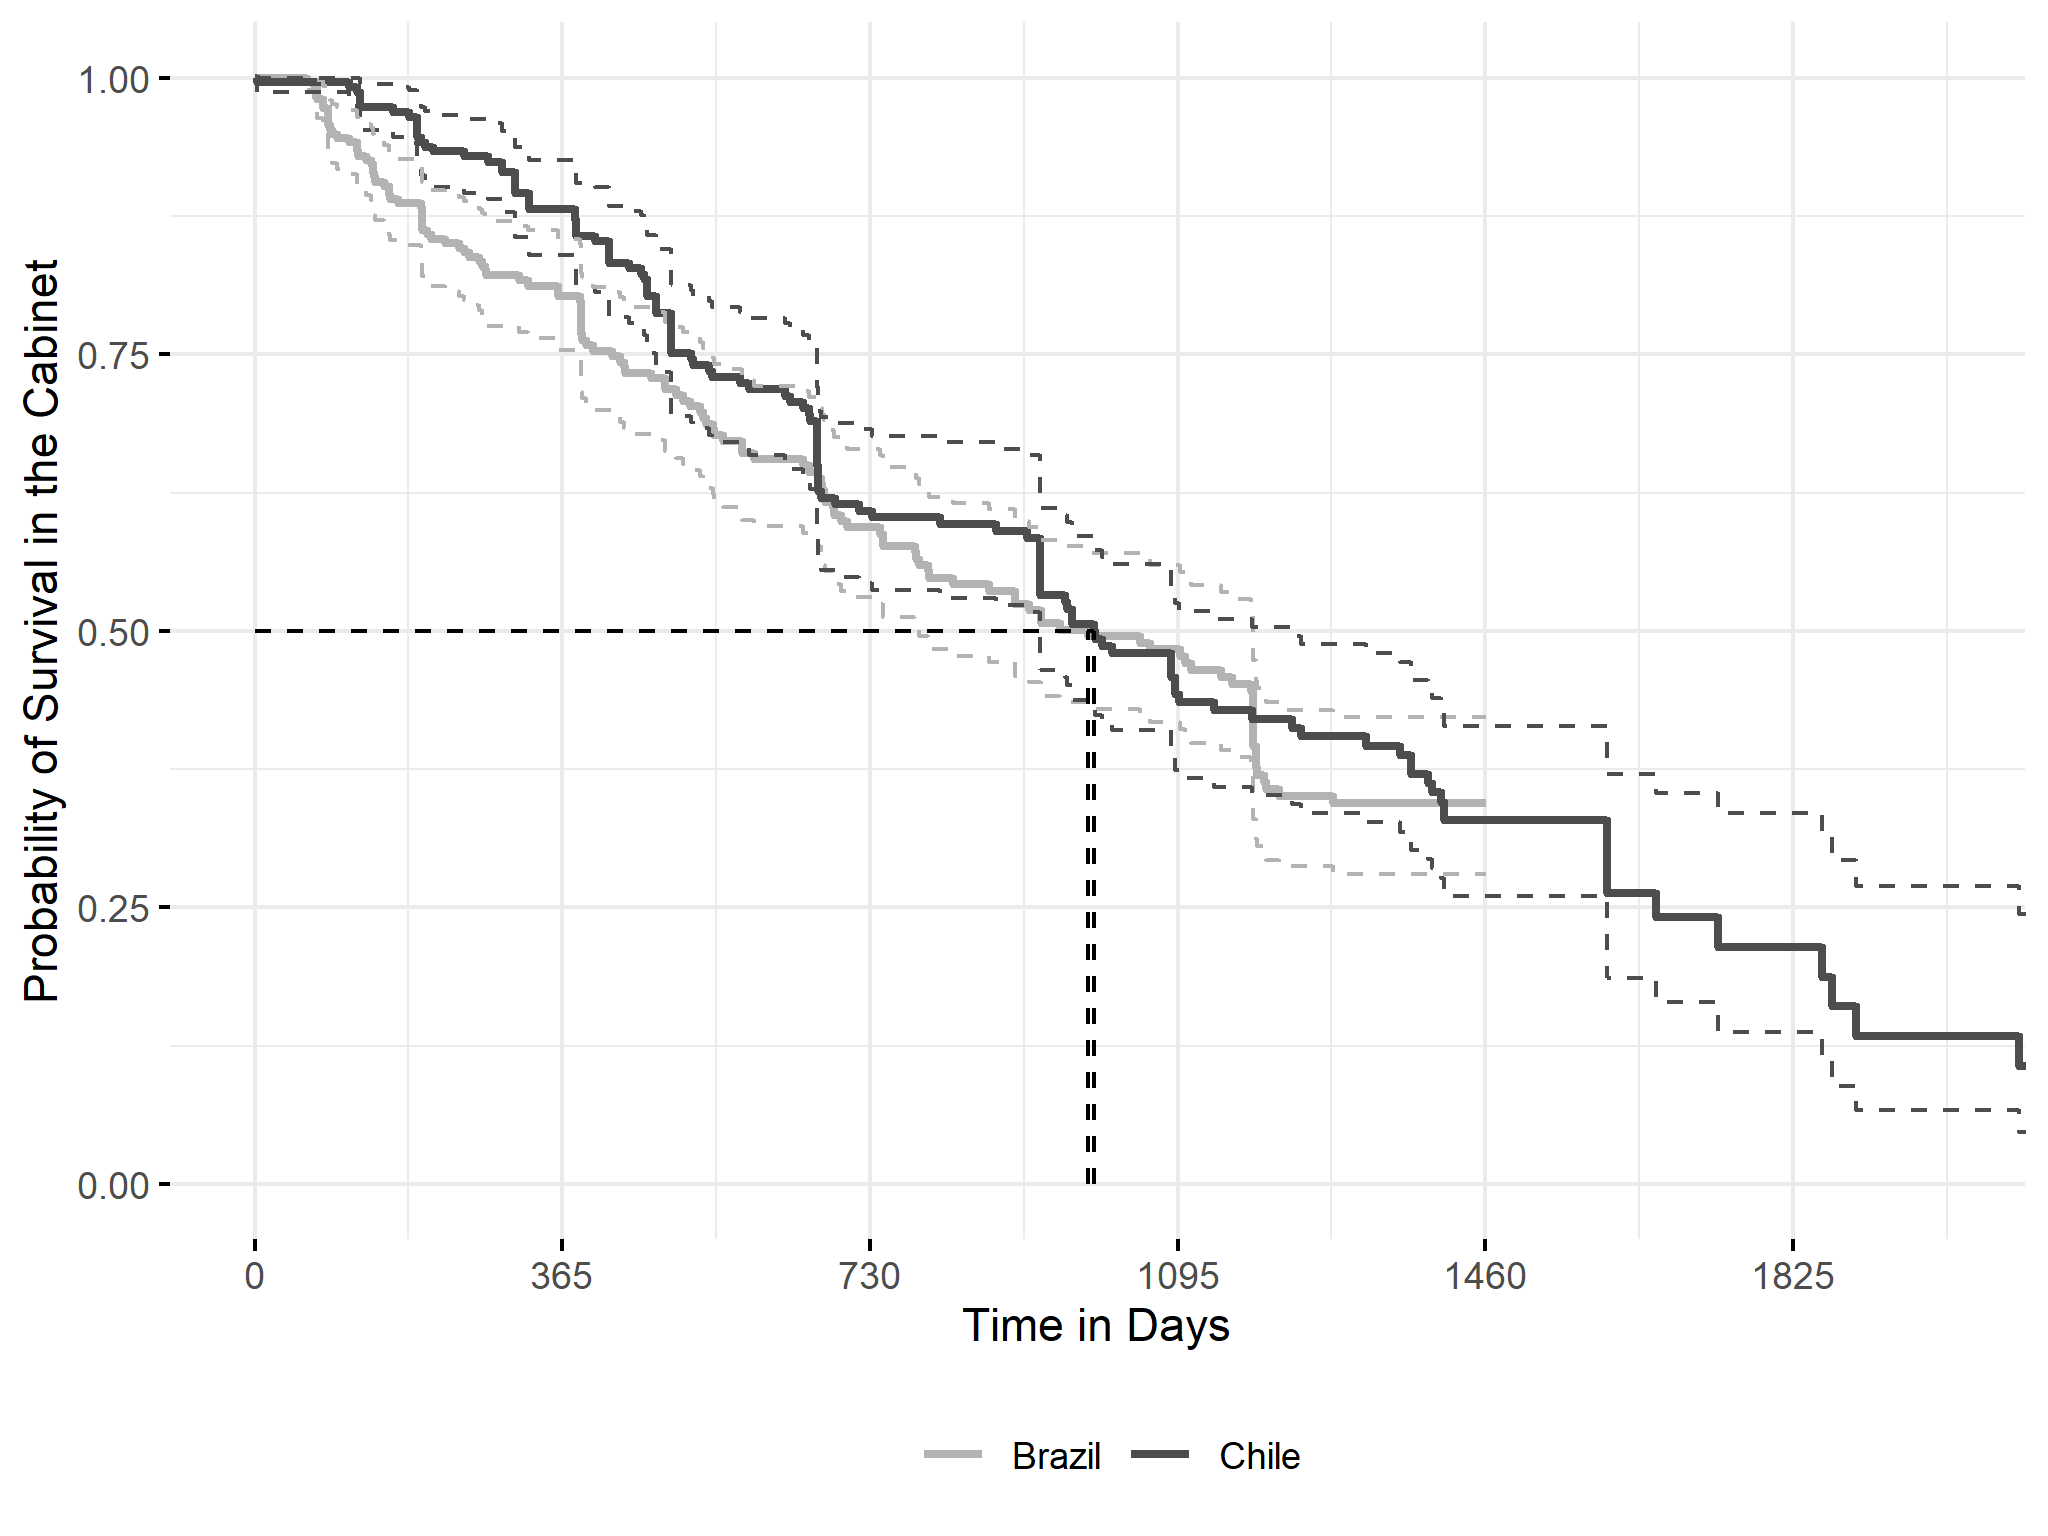
\includegraphics[width=0.49\linewidth]{figures/kaplan_meier} 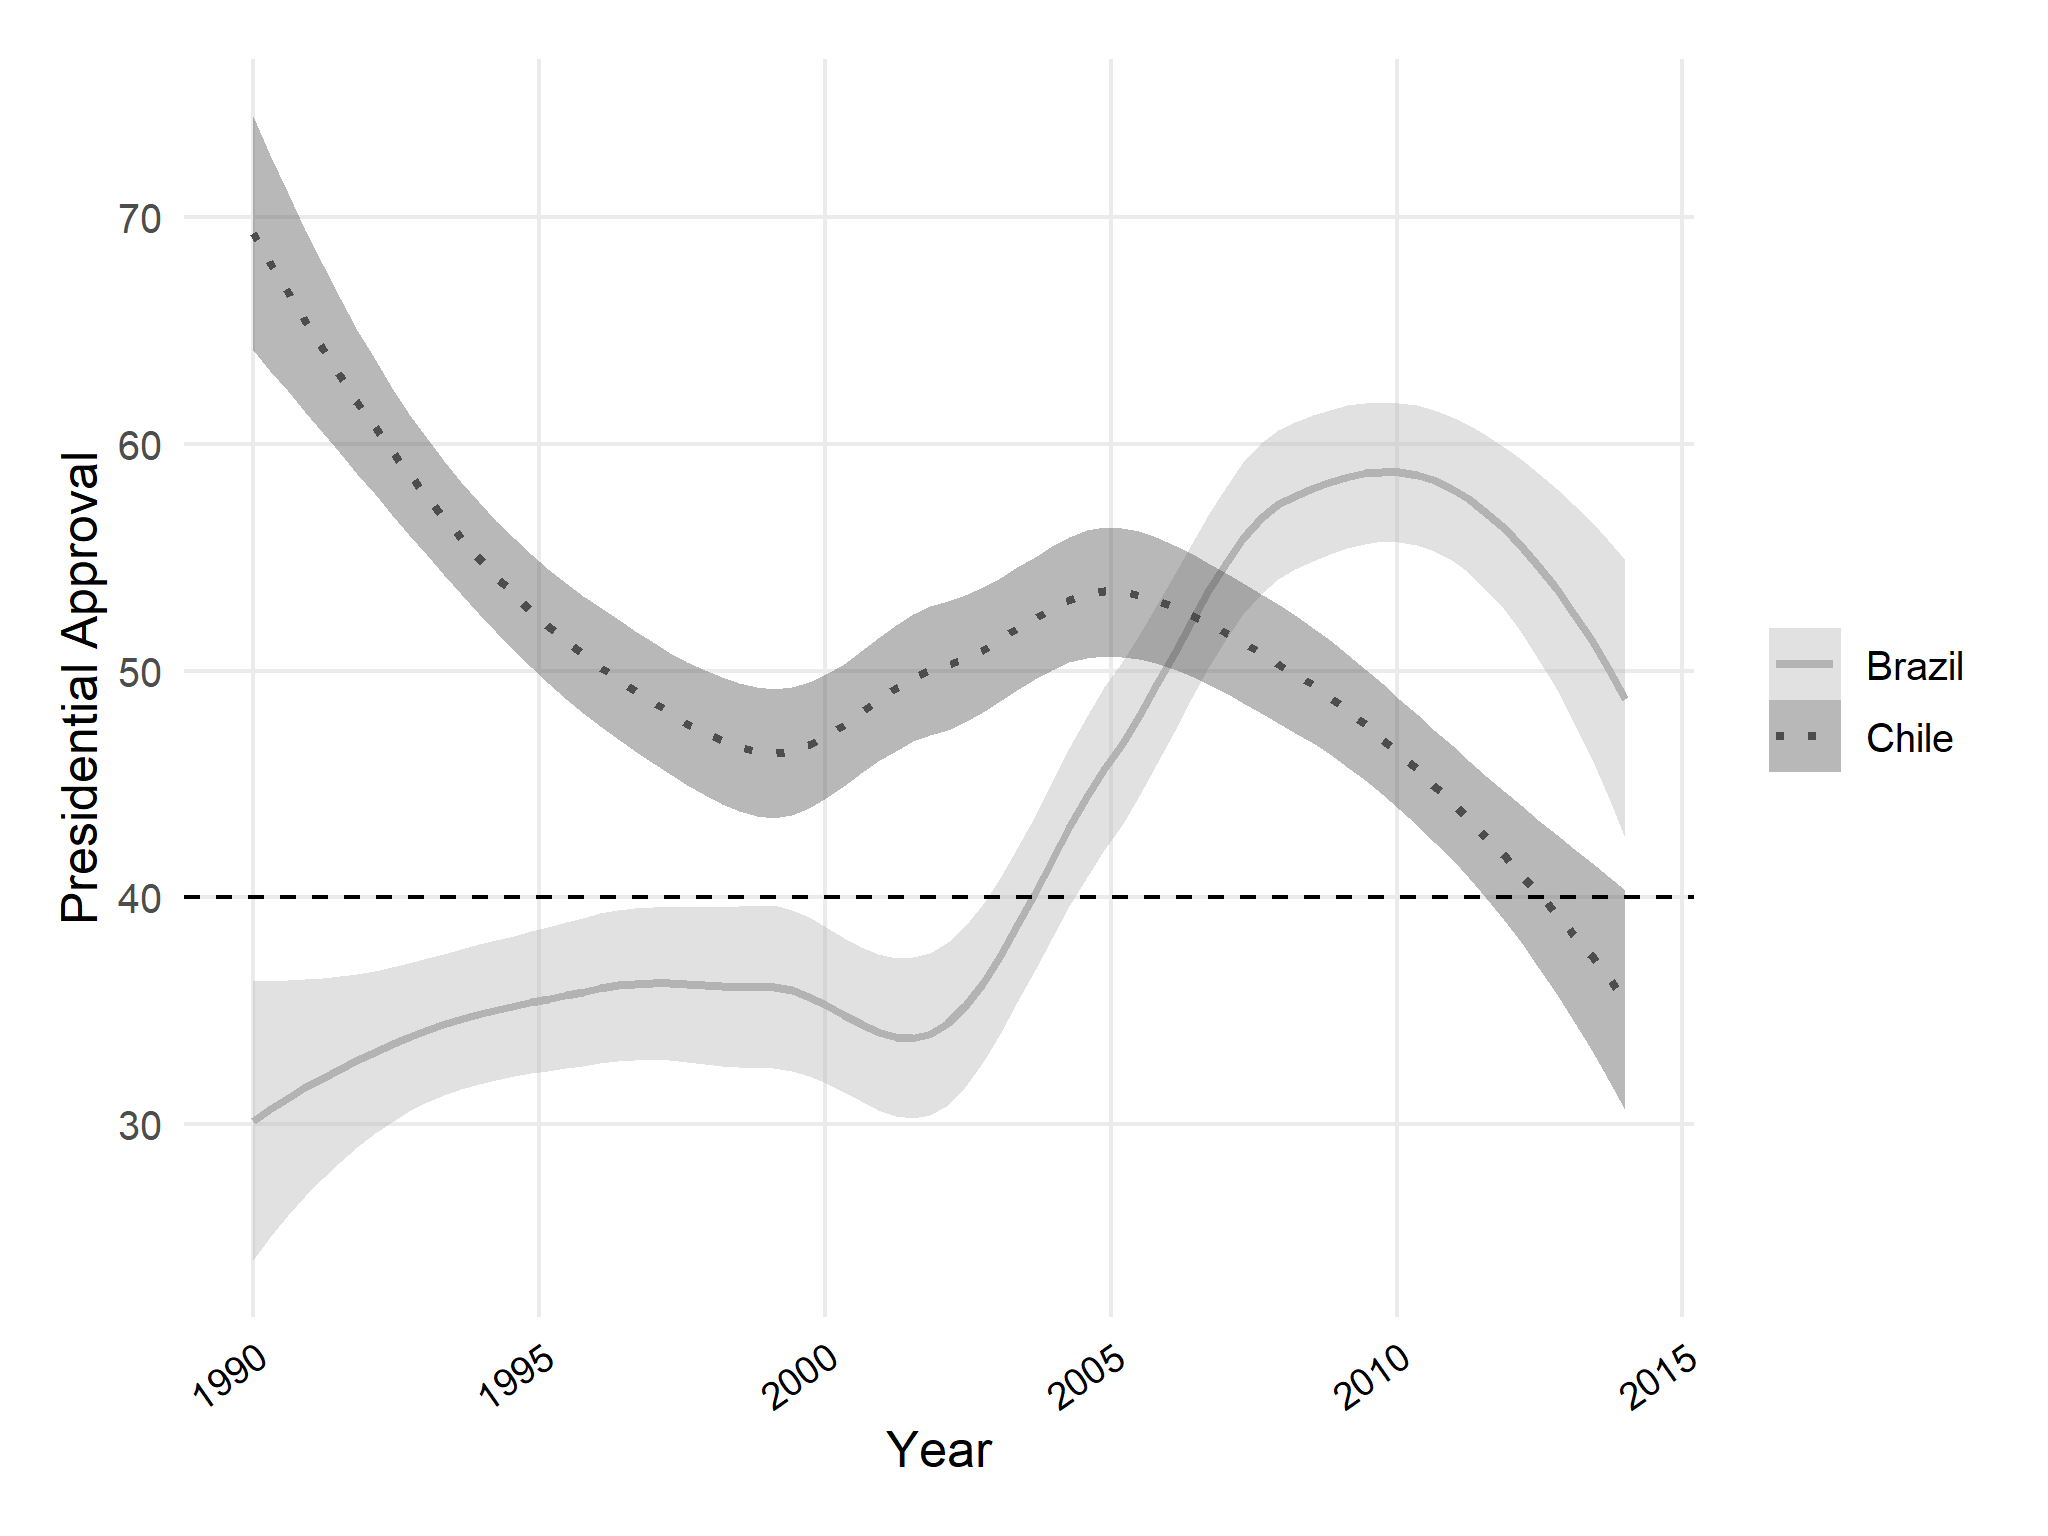
\includegraphics[width=0.49\linewidth]{figures/approval} \\ \vspace{2mm}
%% {\footnotesize Source: Compiled by author.}
\end{figure}

\subsection{Time-Varying Exposure Cox Regressions}
\label{sec3.2}

\bibliographystyle{apalike}
\bibliography{refs/BIB-Ministers-Approval}
\addcontentsline{toc}{section}{References}

\end{document}